\chapter{Truth Discovery}

\todo{Introduction}

\begin{figure}
\centering
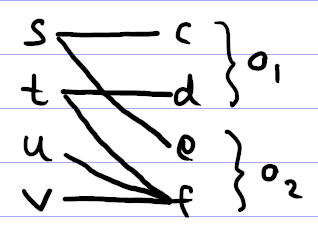
\includegraphics[scale=0.5]{intro_example_new}
\caption{
    \todo{Caption, Tikzify, natural language version, present claims as $c: o =
    v$, bipartite graph with objects just indicated}
}
\label{td_new_fig_intro_example}
\end{figure}

\section{Preliminaries}
\label{td_new_sec_preliminaries}

In this section we give the basic definitions which form our formal framework.

\paragraph{Input.}

Intuitively, a truth discovery problem consists of a number of \emph{sources}
and a number of \emph{objects} of interest. Each source provides a number of
\emph{claims}, where a claim is comprised of an object and a \emph{value}.
Different sources may give conflicting claims by providing different values for
the same object. For simplicity, we only consider categorical values in this
work. Note that while this restriction is made in some approaches in the
literature \todo{citations}, in general truth discovery methods also handle
continuous values \todo{citations}.

To formalise this, let $\S$, $\O$ and $\V$ be infinite, disjoint sets,
representing the possible sources, objects and values. The input to the truth
discovery problem is a \emph{network}, defined as follows.

\begin{definition}
    \label{td_new_def_network}
    A \emph{truth discovery network} is a tuple $N = (S, O, D, R)$, where
    \begin{itemize}
        \item $S \subseteq \S$ is a finite set of \emph{sources}.
        \item $O \subseteq \O$ is a finite set of \emph{objects}.
        \item $D = \{D_o\}_{o \in O}$ are the \emph{domains} of the objects,
              where each $D_o \subseteq \V$ is a finite set of values. We write
              $V = \bigcup_{o \in O}{D_o}$.
        \item $R \subseteq S \times O \times V$ is a set of \emph{reports}.
    \end{itemize}
    such that
    \begin{enumerate}
        \item\label{td_new_item_val_in_domain}
            For each $(s, o, v) \in R$, we have $v \in D_o$.
        \item\label{td_new_item_sources_self_consistent}
            If $(s, o, v) \in R$ and $(s, o, v') \in R$, then $v = v'$.
    \end{enumerate}
\end{definition}

Note that while $\S$, $\O$ and $\V$ are infinite, each network is finite. The
set $R$ is the core data associated with the network: we interpret $(s, o, v)
\in R$ as source $s$ claiming that $v$ is the true value for object $o$.
Constraint \cref{td_new_item_val_in_domain} says that all claimed values are in
the domain of the relevant object. Constraint
\cref{td_new_item_sources_self_consistent} is is a basic consistency requirement:
a source cannot provide distinct values for a single object. That is, a source
provides \emph{at most one value} per object.  Thus, while sources may be in
conflict with \emph{other sources}, they are not in conflict with themselves.
This is a simplifying assumption, and is not universal in the literature; e.g.
\todo{find references}. Nevertheless, we argue the truth discovery problem is
still rich enough when conflicts only arise between distinct sources.

When a network $N$ is understood, we often write $S, O, D$ and $R$ to implicitly
refer to the components of $N$; if necessary we write $S_N, O_N, D_N$ and $R_N$
to make the dependence on $N$ explicit.

A \emph{claim} is a pair $c = (o, v)$, where $o \in O$ and $v \in D_o$. We
write $\obj(c) = o$ in this case, and let $C$ denote the set of all claims in a
network $N$, i.e.
\[
    C = \{(o, v) \mid o \in O, v \in D_o\}.
\]
With slight abuse of notation, we write $(s, c)$ for the report $(s, o, v)$.
Then $R$ can be viewed as a subset of $S \times C$, i.e. a relation between
sources and claims. In fact, we will take this claim-centric view in the
remainder of the paper, with objects and values only playing a role insofar as
they tell us which claims are in conflict with one another.

\begin{example}
    The network illustrated in \cref{td_new_fig_intro_example} is given by $S =
    \{s, t, u, v\}$, $O = \{o_1, o_2\}$, \todo{write when example is polished}
    % \[
    %     N = \{
    %         (s, c), (s, e),
    %         (t, d), (t, f),
    %         (u, f),
    %         (v, f)
    %     \}.
    % \]
\end{example}

\paragraph{Notation.}

We introduce some notation to extract information about a network. For $c \in
C$ and $s \in S$, write
\begin{align*}
    \src_N(c) &= \{s \in S \mid (s, c) \in R\},\\
    \claims_N(c) &= \{c \in C \mid (s, c) \in R\}.
\end{align*}
The set of sources making a claim on object $o$ is
\[
    \src_N(o) = \bigcup\{\src_N(c) \mid c \in C, \obj(c) = o\}.
\]
The set of claims in conflict with a given claim $c = (o, v)$, i.e.  claims for
$o$ with a value other than $v$, is denoted by
\[
    \conflict_N(c) = \{(o, v') \mid v' \in D_o \setminus \{v\}\}.
\]
The ``antisources" of $c$ are then defined to be the sources for claims
conflicting with $c$:
\[
    \antisrc_N(c) = \bigcup\{\src_N(d) \mid d \in \conflict_N(c)\}.
\]

\paragraph{Output.}

With the input defined, we now come to the output of the truth discovery
problem.
The primary goal is to produce as assessment of the trustworthiness of the
sources, and the \emph{true values} for the objects. Approaches differ
regarding values: some truth discovery methods output only a single value for
each object~\cite{li2016,ding_finding_2016,yang_continuous_2018}, whereas
others give as assessment of the believability (or confidence, probability
etc\ldots) of \emph{each claim} $(o,
v)$~\cite{yin2008,pasternack2010,galland2010,zhi2015,zhang_robust_2016,zhang2018}.
We opt for the latter, more general, approach.

On the specific form of these assessments, we face a tension between the social
choice and truth discovery perspectives. In social choice theory, one generally
looks at \emph{rankings}: e.g. the ranking of candidates in an election result
according to a voting rule. Consequently, axioms are generally \emph{ordinal
properties}, which constrain how candidates (for example) compare
\emph{relative to each other}. In contrast, truth discovery methods universally
use \emph{numeric values}. This is more convenient for defining and using truth
discovery methods in practise, and induces a ranking by simply comparing the
numeric scores. However, numeric scores are often not comparable between
different methods (for example, some methods output probabilities, whereas
others are interpreted as weights which may take negative values) and in
general may not carry any semantic meaning at all. This means that meaningful
axioms for truth discovery should not refer to specific numeric scores, but
only the ranking they introduce. \todo{caveat: scores give confidence
estimations.}

We will ultimately take a hybrid approach: our methods and example will be
defined in terms of numeric scores, but the axioms will only refer to ordinal
properties. This approach is summarised succinctly by \textcite{altman2008},
who write of ranking systems: ``We feel that the numeric approach is more
suitable for defining and executing ranking systems, while the global ordinal
approach is more suitable for axiomatic classification."

An \emph{operator} maps each network to score and claim scores.

\begin{definition}
    A \emph{truth discovery operator} $T$ maps each network $N$ to a function
    $T_N: S_N \cup C_N \to \R$.
\end{definition}

Intuitively, the higher the score $T_N(s)$ for a source $s \in S$, the
\emph{more trustworthy} $s$ is, according to $T$ on the basis of $N$.
Similarly, the higher $T_N(c)$ for a claim $c \in C$, the \emph{more
believable} $c$ is deemed to be. We define the source and claim rankings
associated with $T$ and $N$ by
\begin{align*}
    s \sle_N^T s' &\iff T_N(s) \le T_N(s'), \\
    c \cle_N^T c' &\iff T_N(c) \le T_N(c').
\end{align*}
Then $s \sle_N^T s'$ if $s'$ is at least as trustworthy as $s$, and similar for
$\cle_N^T$. Note that $\sle_N^T$ and $\cle_N^T$ are total preorders. We denote
the strict parts by $\slt_N^T$ and $\clt_N^T$ respectively, and the symmetric
parts by $\seq_N^T$ and $\ceq_N^T$. We omit the sub- and super-scripts when
$N$ and $T$ are clear from context.

Given that our axioms will only refer to the rankings produced by operators,
two operators yielding exactly the same rankings -- possibly with different
scores -- appear the same with respect to axiomatic analysis. We say operators
$T$ and $T'$ are \emph{ranking equivalent}, denoted $T \rankequiv T'$, if for
all networks $N$ we have ${\sle_N^T} = {\sle_N^{T'}}$ and ${\cle_N^T} =
{\cle_N^{T'}}$.

In \cref{td_new_sec_example_operators} we will introduce operators defined as
the limit of an iterative procedure. To allow for possible non-convergence we
also consider \emph{partial operators}, which assign a mapping $T_N: S \cup C
\to \R$ for only a subset of networks.

\section{Example Operators}
\label{td_new_sec_example_operators}

In this section we capture several example operators from the literature in our
framework: a baseline \emph{voting} and method its generalisation to
\emph{weighted} voting, \emph{Sums}~\cite{pasternack2010},
\emph{TruthFinder}~\cite{yin2008} and \emph{CRH}~\cite{li2016}. As is the case
with many methods in the literature, the latter three methods operate
iteratively: starting with an initial estimate, scores are repeatedly updated
according to some procedure until convergence. Typically the update procedure
is recursive, with source scores being updated on the basis of the current
claims scores, and vice versa.  To simplify the definition and analysis of such
methods, we will introduce the class of \emph{recursive operators}.

\subsection{Voting}

It is common in the literature to evaluate truth discovery methods against a
non-trust-aware method, such as a simple voting procedure.\footnotemark{} Here
we consider each source to ``vote" for their claims, and claims are ranked
according to the number of votes received, i.e. by $|\src_N(c)|$. While this
ignores the trust aspect of truth discovery entirely, this method will be
useful for us as an axiomatic baseline. For example, axioms which aim to
address the trust aspect should not hold for voting, and an axiom referring to
the ranking of claims may be too strong if it does hold for voting.

\footnotetext{
    This is often called \emph{majority voting} in the truth discovery
    literature (e.g.~\cite{li_survey_2016,xiao_22,li2016}), but using the
    terminology of social choice theory it is better described as
    \emph{plurality voting}.
}

\begin{definition}
    $\voting$ is the operator defined by
    \begin{align*}
        \voting_N(s) &= 1,\\
        \voting_N(c) &= |\src_N(c)|.
    \end{align*}
\end{definition}

Applying $\voting{}$ to the network in \cref{td_new_fig_intro_example}, we have
that all sources rank equally ($s \seq t \seq u \seq v$) and $c \ceq d \ceq e
\clt f$.

The problem with $\voting{}$ is that all reports are equally weighted. If we
have a mechanism by which sources can be weighted by trustworthiness, the idea
behind voting may still have some merit. We define \emph{weighted voting} as
follows.

\begin{definition}
    A \emph{weighting} $w$ maps each network $N$ to a function $w_N: S \to \R$.
    The associated \emph{weighted voting} operator $\wvoting{w}$ is defined by
    \begin{align*}
        \wvoting{w}_N(s) &= w_N(s), \\
        \wvoting{w}_N(c) &= \sum_{s \in \src_N(c)}{w_N(s)}.
    \end{align*}
\end{definition}

Note that a weighting is essentially just half of a truth discovery operator,
where we only output scores for sources. This is completed to an operator
$\wvoting{w}$ by letting the score for a claim be the sum of the weights of its
sources. Note that we allow the possibility of ``untrustworthy" sources with
$w_N(s) < 0$. Reports from such sources \emph{decrease} the credibility of a
claim.

\begin{example}
    \label{td_new_ex_weighted_voting}
    Set
    \[
        w_N(s) = \frac{1}{|\claims_N(s)|}{
            \sum_{c \in \claims_N(s)}{
                |\src_N(c)|
            }
        }.
    \]
    Then the weight assigned to a source $s$ is the average number of sources
    agreeing with the claims of $s$. Taking $N$ from
    \cref{td_new_fig_intro_example}, we have $w_N(s) = 1$, $w_N(t) = 2$,
    $w_N(u) = 3$, $w_N(v) = 3$.  Consequently,
    \begin{align*}
        \wvoting{w}_N(c) &= w_N(s) = 1,\\
        \wvoting{w}_N(d) &= w_N(t) = 2,\\
        \wvoting{w}_N(e) &= w_N(s) = 1,\\
        \wvoting{w}_N(f) &= w_N(t) + w_N(u) + w_N(v) = 8,
    \end{align*}
    yielding the rankings $s \slt t \slt u \seq v$ and $c \ceq e \clt d \clt
    f$. Note that claim $d$ fares better here than with $\voting$ due to its
    association with source $t$, who is more trustworthy than $s$.
\end{example}

As we will see in \todo{section reference}, some operators do not correspond
exactly to a weighting $w$, but give rise to the same rankings. Let us say an
operator $T$ is \emph{weightable} if there exists a weighting $w$ such that $T
\rankequiv \wvoting{w}$. Given that weighted voting expresses a clear
relationship between source and claim scores, this notion will greatly simplify
axiomatic analysis in \todo{section reference}.

\subsection{Recursive Operators}

To capture the mutual dependence between trust in sources and belief in claims,
truth discovery methods generally involve recursive
computation~\cite{pasternack2010,yin2008,yang_probabilistic_2019,du2019,zhang2018,li2016,galland2010,zhi2015}.
Claim scores are updated on the basis of currently estimated source scores,
before claim scores are updated on the basis of the new sources scores. If this
process converges, the limiting scores should be a fixed-point of the update
procedure, reflecting the desired mutual dependence. To formalise this idea, we
define recursive operators.

\begin{definition}
    A \emph{recursive scheme} is a tuple $(\T, T^0, U)$, where
    \begin{itemize}
        \item $\T$ is a set of operators.
        \item $T^0 \in \T$ is the \emph{initial operator}.
        \item $U: \T \to \T$ is the \emph{update function}.
    \end{itemize}
    A recursive scheme \emph{converges} on a network $N$ if for all $z
    \in S \cup C$, the limit $\lim_{n \to \infty}{U^n(T^0)_N(z)}$ exists. The
    \emph{limit} of a recursive scheme is the partial operator $T^*$ defined on
    the networks $N$ on which the scheme converges, given by $T^*_N(z) =
    \lim_{n \to \infty}{U^n(T^0)_N(z)}$.
\end{definition}

The main component of interest here is the update function $U$, which describes
how the scores of one iteration are transformed to obtain scores for the next.
The domain of operators $\T$ is used for technical reasons; for example, some
operators need to exclude the trivial operator in which scores are identically
zero in order for $U$ to be well-defined. We will analyse convergence and
fixed-point properties -- i.e. whether $U(T^*) = T^*$ -- in
\cref{td_new_sec_convergence_fixed_points}. For now, we introduce examples of
recursive operators from the literature.

\paragraph{Sums.}

Sums~\cite{pasternack2010} is a simple and well-known operator adapted from the
\emph{Hubs and Authorities}~\cite{kleinberg1999} algorithm for ranking web
pages. The premise is to extend the linear sum of weighted voting to both claim
and source scores: we update the score of each source as the sum of the scores
of its claims, and update the score of each claim as the sum of the scores of
its sources. To prevent scores from growing without bound, they are normalised
at each iteration by dividing by the maximum score (for sources and facts
separately).

\begin{definition}
    \emph{Sums} is the recursive scheme $(\T, T^0, U)$, where $\T$ is the set
    of all operators, $T^0_N \equiv 1 / 2$, and $U(T) = T'$, with
    \begin{align*}
        T'_N(s) &=
            \frac{1}{Z_S}
            \sum_{c \in \claims_N(s)}{
                T_N(c)
            },
        \\
        T'_N(c) &=
            \frac{1}{Z_C}
            \sum_{s \in \src_N(c)}{
                T'_N(s)
            }.
    \end{align*}
    where $
        Z_S = \max_{t \in S}{
            \left|
                \sum_{c \in \claims_N(t)}{
                    T_N(c)
                }
            \right|
        }
    $ and $
        Z_C = \max_{d \in C}{
            \left|
                \sum_{s \in \src_N(d)}{
                    T'_N(s)
                }
            \right|
        }
    $ are normalisation factors (and we set $T'_N \equiv 0$ if either $Z_S$ or
    $Z_C$ are 0). We write $\sums$ for the associated limit operator.
\end{definition}

Taking the network $N$ from \cref{td_new_fig_intro_example}, one can show that
$\sums_N(s) = 0$, $\sums_N(t) = 1$ and $\sums_N(u) = \sums_N(v) = \sqrt{2} / 2
\approx 0.7071$, giving a source ranking $s \slt u \seq v \slt t$.  For claims,
we have $\sums_N(c) = \sums_N(e) = 0$, $\sums_N(d) = \sqrt{2} - 1 \approx
0.4142$ and $T_N(f) = 1$, giving a claim ranking $c \ceq e \clt d \clt f$. Note
that the claim ranking is identical to that of
\cref{td_new_ex_weighted_voting}. For sources, we see that $t$ moves strictly
upwards in the ranking compared to \cref{td_new_ex_weighted_voting}.
Intuitively, this is because source $t$ claims a superset of the claims of $u$
and $v$, so receives more weight from its claims at each iteration.

\paragraph{TruthFinder.} TruthFinder~\cite{yin2008} is a pseudo-probabilistic
method, and was defined in the first paper to introduce (and coin the phrase)
truth discovery. It is formulated in a setting more general than ours: the
authors suppose claims may \emph{support} each other, as well as conflict, and
that support of conflict may occur to varying degrees. Formally, each pair of
claims $c, c'$ has an ``implication" value $\operatorname{imp}(c \to c') \in
[-1, 1]$, where a negative value implies confidence in $c$ should decrease
confidence in $c'$, and a positive value implies confidence in $c$ should
\emph{increase} confidence in $c'$. In contrast, our framework assumes claims
for the same object are mutually exclusive, so that all implications are
negative. To express TruthFinder in our framework, we take
$\operatorname{imp}(c \to c')$ to be $-\lambda$ if $c$ and $c'$ have the same
object and $0$ otherwise, for some fixed parameter $0 \le \lambda \le 1$.

\begin{definition}
    Given parameters $0 \le \rho, \lambda \le 1$, and $0 < \gamma < 1$,
    \emph{TruthFinder} is the recursive scheme $(\T, T^0, U)$, where $\T$ is
    the set of operators with $0 < T_N(s) < 1$ for all $N$ and $s \in S$ with
    $\claims_N(s) \ne \emptyset$, $T^0 \equiv 0.9$, and $U(T) = T'$, with
    \begin{align}
        \label{td_new_eqn_truth_finder_claim_update}
        T'_N(c) &= \left[
            1 +
            \frac{
                \prod_{s \in \src_N(c)}{(1 - T_N(s))^\gamma}
            }{
                \prod_{t \in \antisrc_N(c)}{(1 - T_N(t))^{\gamma\rho\lambda}}
            }
        \right]^{-1}, \\
        T'_N(s) &= \sum_{c \in \claims_N(s)}{
            \frac{T'_N(c)}{|\claims_N(s)|}
        }.
    \end{align}
    We write $\truthfinder$ for the associated limit operator.
\end{definition}

We refer the reader to the original TruthFinder paper~\cite{yin2008} for the
interpretation of $\rho$ and $\gamma$. As described above, $\lambda$ controls
the amount to which conflicting claims play a role in the evaluation of a given
claim. Of special interest is the case $\lambda = 0$, in which the denominator
in \cref{td_new_eqn_truth_finder_claim_update} is $1$. Note that in
\cref{td_new_eqn_truth_finder_claim_update} we have unfolded the definitions of
\textcite{yin2008} in order to obtain a single expression of $T'_N(c)$ in terms
of the $T_N(s)$.

Let us return again to the network in \cref{td_new_fig_intro_example}. We take
parameters $\rho = 0.5$ and $\gamma = 0.3$ (as per the experimental setup of
\textcite{yin2008}) and $\lambda = 0.5$. Assuming that TruthFinder does indeed
converge on this network -- as it appears to do empirically -- we have
$\truthfinder_N(s) \approx 0.5067$, $\truthfinder_n(t) \approx 0.6590$ and
$\truthfinder_N(u) = \truthfinder_N(v) = 0.7510$, which gives the ranking $s
\slt t \slt u \seq v$ on the sources. We have $\truthfinder_N(c) \approx
0.5328$, $\truthfinder_N(d) \approx 0.5670$, $\truthfinder_N(e) \approx 0.4807$
and $\truthfinder_N(f) \approx 0.7510$, which gives the ranking $e \clt c \clt
d \clt f$ on the claims. Note that the source ranking coincides with that of
\cref{td_new_ex_weighted_voting}, and the claim ranking refines that of
\cref{td_new_ex_weighted_voting} and Sums by ranking $e$ \emph{strictly} worse
than $c$. Intuitively, this occurs because $e$ has more sources reporting the
conflicting claim (namely, $f$) than $c$ does. If we instead take $\lambda =
0$, so that sources for conflicting claims are not considered, then the ranking
reverts to $c \ceq e \clt d \clt f$.

\paragraph{CRH.} Standing for ``Conflict Resolution on Heterogeneous Data", CRH
is an optimisation-based framework for truth discovery~\cite{li2016}. It is
again set in a more general framework, in which a metric $d_o$ is available to
measure the distance between values in $D_o$, for each object $o$. The
optimisation problem jointly chooses weights for each source and a value for
each object, such that the weighted sum of $d_o$-distances from each source's
claim on $o$ is minimised.

To express CRH in our framework we use the ``probabilistic" encoding of
categorical variables as described in \cite[\sectionsymbol{2.4.1}]{li2016},
where each categorical value is represented as a one-hot vector.

\begin{definition}
    \emph{CRH} is the recursive scheme $(\T, T^0, U)$, where $\T$ is
    \todo{what?}, $T^0$ is given by
    \[
        T^0_N(s) = 0, \qquad
        T^0_N(c) = \frac{|\src_N(c)|}{|src_N(\obj(c))|},
    \]
    and $U(T) = T'$, where
    \begin{align*}
        \alpha_s &= \sum_{c \in \claims_N(s)}{
            \left(
                (T_N(c) - 1)^2
                +
                \sum_{d \in \conflict_N(c)}{
                    T_N(d)^2
                }
            \right)
        }, \\
        T'_N(s) &= -\log\frac{\alpha_s}{\sum_{t \in S}{\alpha_t}}, \\
        T'_N(c) &=
            \frac{\sum_{s \in \src_N(c)}{T'_N(s)}}{\sum_{t \in S}{T'_N(t)}}.
    \end{align*}
\end{definition}

\todo{Finish writing, example.}

\todo{Table of rankings of each example on the intro network.}

\section{The Axioms}

Having laid out the formal framework, we now introduce axioms for truth
discovery. Such axioms are formal properties an operator may satisfy, which
encode intuitively desirable behaviour. Many of our axioms are adaptations of
axioms for various problem in social choice theory (e.g. from
voting~\cite{zwicker2016voting} and ranking systems~\cite{altman2008}), in
which the axiomatic method has seen great success. We also consider standard
social choice axioms which are \emph{not} desirable for truth discovery, to
highlight the differences with classical problems such as voting. We will later
revisit the example operators of the previous section to see to what extend our
axioms hold in practise.

\subsection{Coherence}

The guiding principle of truth discovery is that claims backed by trustworthy
sources should be believed, and sources making believable claims are
trustworthy. All truth discovery methods aim to implement this principle to
some extent, and the examples of \cref{td_new_sec_example_operators} illustrate
several different approaches.

We aim to formulate this principle axiomatically as a \emph{coherency} property
relating the source ranking $\sle$ and the claim ranking $\cle$: sources making
higher $\cle$-ranked claims should rank highly in $\sle$, and vice versa. To do
so we adapt the idea behind the \emph{Transitivity} axiom of
\textcite{altman2008} for ranking systems.

Now, a difficulty arises when considering how to compare the claims of two
sources. For a simple example, suppose sources have either \emph{low},
\emph{medium} or \emph{high} trustworthiness. How should we rank a claim $c$
with one \emph{medium} sources versus a claim $d$ with a \emph{low} and a
\emph{high} source? In some situations we may want to prioritise the number of
claims, so that $d$ is preferred. In others we may want to avoid trusting
\emph{low} sources as much as possible, so that $c$ is preferred. The third
option of ranking $c$ and $d$ equally believable is also reasonable.

To avoid these ambiguous cases, we focus on scenarios where there is an
``obvious" ordering between two sets of claims (or sources). For example,
consider the network depicted in \cref{td_new_fig_coherence_intro}. Suppose an
operator gives a source ranking $s \slt u \slt t \slt v$. Note that claims $c$
and $d$ have the same number of sources. Moreover, we can pair up these sources
one-to-one such that the source for $c$ is less trustworthy than the
corresponding source for $d$: we have $s \slt u$ and $t \slt v$. On aggregate,
we may reasonably say that $\src_N(c)$ is less trustworthy (with respect to
$\sle$) than $\src_N(d)$. We should therefore have $c \clt d$; any operator
violating this has failed to realise the dependence between source
trustworthiness and claim believability. Similarly, this reasoning can be
applied to the set of claims from two sources.

\begin{figure}
    \centering
    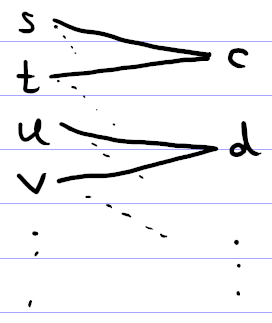
\includegraphics[scale=0.5]{coherence_intro}
    \caption{
        Network illustrating \axiomref{Coherence}.
    }
    \label{td_new_fig_coherence_intro}
\end{figure}

This will form the basis of our first set of axioms. First, we formalise the
above idea of a one-to-one correspondence respecting a ranking.

\begin{definition}
    If $\le$ is a relation on a set $X$ and $A, B \subseteq X$, then $A$
    \emph{precedes $B$ pairwise} with respect to $\le$ if
    \begin{equation}
        \label{td_new_eqn_pwo}
        \exists f: A \to B \text{ bijective s.t. }
        \forall x \in A:\ x \le f(x).
    \end{equation}
    Say $A$ \emph{strictly precedes $B$} if $A$ precedes $B$ but $B$ does not
    precede $A$.
\end{definition}

If $f$ satisfies the condition in \cref{td_new_eqn_pwo}, we say $f$
\emph{witnesses} the fact that $A$ precedes $B$, and write
$\witprec{f}{A}{B}{\le}$.  Note that if $\le$ is a preorder on $X$, the
``precedes pairwise" relation is a preorder on $2^X$.  Indeed, it is reflexive
(by considering the identity map $A \to A$, for each $A \subseteq X$) and
transitive (if $\witprec{f}{A}{B}{\le}$ and $\witprec{g}{B}{C}{\le}$, then
$\witprec{g \circ f}{A}{C}{\le}$). The strict pairwise order associated has a
natural interpretation, as we now prove: there must exists some $x$ in
\cref{td_new_eqn_pwo} for which the comparison is strict.

\begin{proposition}
    \label{td_new_prop_pwo_strict_part}
    Suppose $X$ is finite and $\le$ is a total preorder on $X$. Then $A$
    strictly precedes $B$ pairwise with respect to $\le$ if and only if there
    is $\witprec{f}{A}{B}{\le}$ such that there is some $x_0 \in A$ with $x_0 <
    f(x_0)$.
\end{proposition}

We need a  preliminary lemma.

\begin{lemma}
    \label{td_new_lemma_pwo_strict_helper}
    Suppose $\le$ is a total preorder on a finite set $X$ and $f: X \to X$ is
    an injective mapping such that $x \le f(x)$ for all $x \in X$. Then $x
    \approx f(x)$ for all $x$.
\end{lemma}

\begin{proof}
    Take $x \in X$. Consider the sequence of iterates $(f^n(x))_{n \ge 1}$.
    Since this is an infinite sequence taking values in a finite set, there
    must be some point at which the sequence repeats, i.e. there are $n, k \ge
    1$ such that $f^n(x) = f^{n + k}(x)$. Then $f(f^{n - 1}(x)) = f(f^{n + k -
    1}(x))$, so injectivity gives $f^{n - 1}(x) = f^{n + k - 1}(x)$. Repeating
    this argument, we find $x = f^0(x) = f^k(x)$. By hypothesis, $f(x) \le
    f^k(x)$, i.e.  $f(x) \le x$. Since $x \le f(x)$ also, this gives $x \approx
    f(x)$ as required.
\end{proof}

\begin{proof}[Proof of \cref{td_new_prop_pwo_strict_part}]
    ``if": Clearly $A$ precedes $B$. Suppose for contradiction that this is not
    strict. Then there is some $\witprec{g}{B}{A}{\le}$. Note that $g \circ f$
    is a bijection $A \to A$, and for all $x \in X$ we have $x \le f(x) \le
    g(f(x))$. By \cref{td_new_lemma_pwo_strict_helper}, $x \approx g(f(x))$. In
    particular, we have $f(x_0) \le g(f(x_0)) \approx x_0$, but this
    contradicts $x_0 < f(x_0)$.

    ``only if": Suppose $A$ strictly precedes $B$. Then there is some
    $\witprec{f}{A}{B}{\le}$. Note that $f^{-1}$ is a bijection $B \to A$.
    Since $B$ does not precede $A$, there must be some $y_0 \in B$ such that
    $y_0 \not\le f^{-1}(y_0)$. By totality of $\le$, we get $f^{-1}(y_0) <
    y_0$. Taking $x_0 = f^{-1}(y_0)$, we are done.
\end{proof}

We are now ready to state our first two axioms.

\begin{axiomlist}
\begin{axiom}[\claimcoherence{}]
    If $\src_N(c)$ strictly precedes $\src_N(c')$ pairwise with respect to
    $\sle_N^T$, then $c \clt_N^T c'$.
\end{axiom}
\begin{axiom}[\sourcecoherence{}]
    If $\claims_N(s)$ strictly precedes $\claims_N(s')$ pairwise with respect to
    $\cle_N^T$, then $s \slt_N^T s'$.
\end{axiom}
\end{axiomlist}

In words, \claimcoherence{} says that whenever we can pair up the sources for
$c$ and $c'$ can be paired up so that each source for $c$ is less trustworthy
than the corresponding source for $c'$ (and \emph{strictly} less, for at least
one pair of sources), then $c$ is strictly less believable than $c'$. Likewise,
\sourcecoherence{} says that if the claims of $s$ and $s'$ can be paired up
with the claims for $s$ less believable than the claims for $s'$, then $s$ is
strictly less trustworthy than $s'$.

\begin{example}
    \label{td_new_ex_coherence_ilustration}
    Consider the network $N$ from \cref{td_new_fig_intro_example} again, and
    consider Sums. Recall that $\sums$ gives the source ranking $s \slt u \seq
    v \slt t$, and claim ranking $c \ceq e \clt d \clt f$.

    Note that $\src_N(c) = \{s\}$ and $\src_N(d) = \{t\}$. Since $s \slt t$, we
    have that $\{s\}$ strictly precedes $\{t\}$ with respect to $\sle$.
    \claimcoherence{} therefore requires that $c \clt d$. Indeed, this does
    hold.

    For \sourcecoherence{}, note that $\claims_N(s) = \{c, e\}$ and
    $\claims_N(t) = \{d, f\}$. Since $c \clt d$ and $e \clt f$, we see that
    $\claims_N(s)$ strictly precedes $\claims_N(t)$ with respect to $\cle$.
    Accordingly, \sourcecoherence{} requires $s \slt t$, which does hold.

    So, $\sums$ satisfies both coherence properties for this specific network.
    We will analyse $\sums$ and the other example in general in \todo{section
    reference}.
\end{example}

The reader may wonder why we only consider the \emph{strict} pairwise relation
in \claimcoherence{} (and \sourcecoherence{}). An alternative axiom might
require that $c \cle c'$ whenever $\src_N(s)$ precedes $\src_N(s')$ with
respect to $\sle$ (not necessarily strictly). However, this property implies
that $c \ceq c'$ whenever $\src_N(c) = \src_N(c')$. We have already seen an
example operator where this does not hold: TruthFinder ranks $e \clt c$ in the
network $N$ from \cref{td_new_fig_intro_example}, but $\src_N(c) = \src_N(e) =
\{s\}$. Intuitively, $c$ and $d$ are ``tied" when it come to the quality of
their own sources, but there are fewer sources \emph{disagreeing} with $c$ (the
``antisources") than $e$. Stating our coherence properties in the strict form
permits an operator to consider antisources in cases where there is no clear
comparison on the basis of sources alone. \todo{What about justification for
the strict form of \sourcecoherence{}? Symmetry will already require equal
ranking for sources with the same claims.}

This discussion leads to a new interpretation of mutual-dependence principle of
truth discovery: claims refuted by trustworthy sources should \emph{not} be
believed. We formulate this as an axiom.

\begin{axiom}[\anticoherence{}]
    If $\antisrc_N(c)$ strictly precedes $\antisrc_N(c')$ pairwise with respect
    to $\sle_N^T$, then $c' \clt_N^T c$.
\end{axiom}

Recall that $\antisrc_N(c)$ are the sources making some claim which conflicts
with $c$. Thus, \anticoherence{} says that if the antisources for $c'$ are more
trustworthy than those of $c$, then $c$ is strictly more believable than $c'$.
While both \claimcoherence{} and \anticoherence{} are reasonable in isolation,
there is an inherent tension between them: \claimcoherence{} looks at the
sources supporting a claim, whereas \anticoherence{} looks at sources refuting
a claim. We explore this tension in \todo{section reference}, where we provide
an impossibility result showing that both cannot hold at the same, alongside
some other reasonable properties.

\todo{Limitation: we can only compare sources/claims with the same number of
claims/sources. Signpost if we end up improving this later by considering extra
trustworthy sources/claims.}

\subsection{Symmetry}

A standard class of axioms in social choice theory are \emph{symmetry
properties}. In voting, for example, symmetry with respect to voters says that
a voting rule should not care about the ``names" of the voters: if voters $i$
and $j$ swap their ballots, the election result remains the same (this is
called \emph{anonymity} in the literature). Similarly, symmetry with respect to
candidates says that if we re-label candidates, the outcome remains the same up
to re-labelling (this is called \emph{neutrality}). In general, symmetry
requires that the output of some process depends only on \emph{structural}
features of the input, not the specific ``names" of the entities involved.

For truth discovery, we can consider symmetry with respect to sources, objects
and claims. The central concept is an \emph{isomorphism} between networks.

\begin{definition}
    An \emph{isomorphism} between networks $N$ and $N'$ is mapping $F: S \cup O
    \cup C \to S' \cup O' \cup C'$ such that
    \begin{enumerate}
        \item $\restrict{F}{S}$, $\restrict{F}{O}$ and $\restrict{F}{C}$ are
              bijections $S \to S'$, $O \to O'$ and $C \to C'$, respectively.
        \item For all $s \in S$ and $c \in C$: $(s, c) \in R$ iff $(F(s), F(c))
              \in R'$.
        \item For all $c \in C$, $\obj(F(c)) = F(\obj(c))$.
    \end{enumerate}
\end{definition}

That is, $F$ is a one-to-one correspondence between the sources, objects and
claims of $N$ and their $N'$ counterparts, which respects the structure of the
network. One can easily check that we also have $F(\src_N(c)) =
\src_{N'}(F(c))$ and $F(\claims_N(s)) = \claims_{N'}(F(s))$.
%
The symmetry axiom says an operator should not distinguish isomorphic networks.

\begin{axiom}[\symmetry{}]
    If $F$ is an isomorphism between $N$ and $N'$, then
    $s \sle_N^T s'$ iff $F(s) \sle_{N'}^T F(s')$ and $c \cle_N^T c'$ iff $F(c)
    \cle_{N'}^T F(c')$.
\end{axiom}

\begin{figure}
\centering
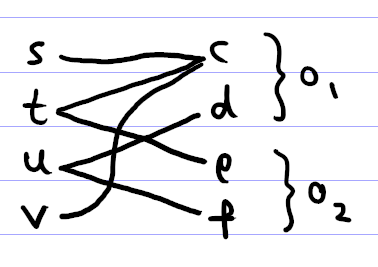
\includegraphics[scale=0.5]{symmetry_example}
\caption{
    A network isomorphic to the one shown in \cref{td_new_fig_intro_example}.
}
\label{td_new_fig_symmetry_example}
\end{figure}

We illustrate \symmetry{} with an example.

\begin{example}
    Consider the network $N$ from \cref{td_new_fig_intro_example} and $N'$ from
    \cref{td_new_fig_symmetry_example}, where we take the sources, objects and
    domains to be the same in both networks. Then $N$ and $N'$ are isomorphic
    via the mapping $F$ expressed in cycle notation as $(suv)(cf)(de)(o_1o_2)$.
    For example, $s$ plays the same role in $N$ as $u$ in $N'$, $c$ plays the
    same role in $N$ as $f$ in $N'$, the role of objects $o_1$ and $o_2$ are
    swapped, etc. \symmetry{} requires that the source and claim rankings in
    $N'$ are already determined by the rankings of $N$.  For example, if the
    source ranking in $N$ is $s \slt_N u \seq_N v \slt_N t$, we must have $u
    \slt_{N'} v \seq_{N'} s \slt_{N'} t$.
\end{example}

An \emph{automorphism} is an isomorphism $F$ from a network $N$ to itself. For
example, $F$ which swaps $u$ and $v$ in $N$ from
\cref{td_new_fig_intro_example} is an automorphism, since $u$ and $v$ play
exactly the same role in $N$. \symmetry{} implies that $u \seq v$, and in fact
this holds more generally.

\begin{proposition}
    If $F$ is an automorphism on $N$ and $T$ satisfies \symmetry{}, then $s
    \seq_N^T F(s)$ and $c \ceq_N^T F(c)$, for all $s \in S$ and $c \in C$.
\end{proposition}

\begin{proof}
    We show $s \seq_N^T F(s)$ for all sources $s$; the result for claims is
    similar.
    %
    Take $s \in S$. Since $S$ is finite and $F$ restricts to a bijection $S \to
    S$, an argument identical to the one in the proof of
    \cref{td_new_lemma_pwo_strict_helper} shows there is some $k \ge 1$ such
    that $s = F^k(s)$.

    First suppose $s \sle_N^T F(s)$. By \symmetry{} we may apply $F$ to both
    sides; doing so repeatedly yields $F^n(s) \sle_N^T F^{n+1}(s)$ for all $n
    \ge 1$. By transitivity of $\sle_N^T$, we get $F(s) \sle_N^T F^n(s)$.
    Taking $n = k$ gives $F(s) \sle_N^T F^k(s) = s$, so $s \seq_N^T F(s)$.

    Now suppose $F(s) \sle_N^T s$. By an identical argument, $F^n(s) \sle_N^T
    F(s)$ for all $n \ge 1$; taking $n = k$ gives $s \sle_N^T F(s)$, so $s
    \seq_N^T F(s)$ again.

    Since $\sle_N^T$ is total these cases are exhaustive, and we are done.

\end{proof}

\subsection{Independence}

Another common class of axioms in social choice theory are \emph{independence}
axioms, which require that some aspect of the output is independent of
``irrelevant" parts of the input. We introduce three such axioms: an adaptation
of independence in classical social choice theory, a structural independence
property concerning unions of disjoint networks, and a property concerning the
marginal effects of one set of sources over another.

\paragraph{Classical independence.}

Arrow's \emph{Independence of Irrelevant Alternatives} in voting
theory~\cite{arrow1952} is the original independence axiom in classical social
choice theory. Roughly speaking, it says that the ranking of candidates $A$ and
$B$ should depend only on the individual rankings of $A$ and $B$, not on any
``irrelevant" alternative $C$. It has been adapted to several settings in which
the axiomatic method has been applied; perhaps closest to our setting is
judgment aggregation, where independence requires the collective acceptance of
a report $\phi$ does not depend on how the individuals accept or reject some
other report $\psi$~\cite{endriss2016ja}.

This can be easily re-stated in our framework: the ranking of claims $c$ and
$d$ should depend only on the sources reporting $c$ and $d$, not on the sources
for other claims. However, this axiom is clearly \emph{undesirable} for truth
discovery. Indeed, consider again the network $N$ from
\cref{td_new_fig_intro_example}. As we have argued informally, claim $c$ is
intuitively weaker than $d$ because how of their respective sources interact
with other claims in the network. Nevertheless, we state this axiom as a point
of comparison with classical social choice problems such as voting.

\begin{axiom}[\classicalindependence{}]
    If $\src_N(c) = \src_{N'}(d)$ and $\src_N(d) = \src_{N'}(d)$, then $c
    \cle_N^T d$ iff $c \cle_{N'}^T d$.
\end{axiom}

That is, if $c$ and $d$ have the same sources in $N$ and $N'$, they have the
same relative ranking in both networks. The undesirability of
\classicalindependence{} will be formalised in \todo{section reference}, where
we show it implies voting-like behaviour and obtain an impossibility result.
\todo{check we actually do this.}

\paragraph{A structural property.}

The problem with \classicalindependence{} is that it ignores the indirect ways
in which claims interact in a network; for example, by referring to the same
object or having common sources. Our next axiom accounts for such interactions
by considering networks with \emph{disjoint sub-networks}, such as the one
shown in \todo{figure}. Intuitively, while the sources and claims within a
sub-network may interact in complex ways, the fact that the sub-networks have
no sources or objects in common means there is no interaction \emph{between}
them. Accordingly, we should have that the ranking for one does not depend on
the other. We formalise this by considering unions of \emph{disjoint
networks}.\footnotemark{}

\footnotetext{
    Note that it is possible to define the disjoint union of an arbitrary
    collection of (not necessarily disjoint) networks in a manner similar to
    the disjoint union of a collection of sets $\bigsqcup_{i \in I}{X_i}$, but
    we do not need this generality here.
}

\begin{definition}
    Networks $N$ and $N'$ are \emph{disjoint} if $S \cap S' = \emptyset$ and $O
    \cap O' = \emptyset$. For $N, N'$ disjoint, their \emph{union} is the
    network $N \sqcup N' = (S \cup S', O \cup O', \hat{D}, R \cup R')$, where
    $\hat{D}_o = D_o$ for $o \in O$, and $\hat{D}_o = D'_o$ for $o \in O'$.
\end{definition}

Note that if $N$ and $N'$ are disjoint, it follows that $C \cap C' = \emptyset$
also.
%
The following axiom says that the ranking of sources and claims is unaffected
by the addition of a disjoint network.

\begin{axiom}[\disjointindependence{}]
    If $N$ and $N'$ are disjoint, $s, t \in S$, and $c, d \in C$, then
    $s \sle_N^T t$ iff $s \sle_{N \sqcup N'}^T t$ and $c \cle_N^T d$ iff $c
    \cle_{N \sqcup N'}^T d$.
\end{axiom}

\todo{explanation on example.}

\todo{if bothered, explain graph-theoretic interpretation in terms of connected
components.}

\paragraph{Marginal independence.}

\todo{intro}

\begin{axiom}[\marginalindependence{}]
    If $\src_N(c) = X \cup Y$, $\src_N(d) = X \cup Z$, $\src_N(c') = X' \cup
    Y$ and $\src_N(d') = X' \cup Z$, then $c \cle_N^T d$ iff $c' \cle_N^T d'$.
\end{axiom}

\subsection{Monotonicity}

For $s \in S$ and $c \in C$, let $N \cup (s, c)$ denote the network $(S, O, D,
R')$, where $R' = R \cup \{(s, c)\}$. Note that $N \cup (s, c)$ may fail to be
a network if $s$ already makes a claim for $\obj(c)$ in $N$.

\begin{axiom}[\naiveposresp{}]
    Suppose $s \notin \src_N(\obj(c))$. Then for all $d \in C \setminus \{c\}$,
    $d \cle_N^T c$ implies $d \clt_{N + (s, c)}^T c$.
\end{axiom}

% \begin{axiom}[\singleobjectposresp{}]
%     Suppose there is $o \in O$ such that $\src_N(o') = \emptyset$ for all $o'
%     \ne o$. Then for all $s, c$ and $d \ne c$, $c \cle_N^T d$ implies $c
%     \clt_{N + (S, c)}^T d$.
% \end{axiom}

\begin{axiom}[\freshposresp{}]
    Suppose $\claims_N(s) = \emptyset$. Then for all $c \in C$ and $d \in C
    \setminus \{c\}$, $d \cle_N^T c$ implies $d \clt_{N + (s, c)}^T c$.
\end{axiom}

\begin{definition}
    Given a network $N$ and operator $T$, we define relations $\mrelex$ and
    $\mrelfa$ on $2^S$ by
    \begin{align*}
        Y \mrelex Y &\text{ iff }
            \exists X \subseteq S, c, d \in C \text{ s.t. }
                \src_N(c) = X \cup Y, \src_N(d) = X \cup Z \\ &\qquad \text{ and }
                c \cle_N^T d \\
        % Y \mrelfa Y &\text{ iff }
        %     \forall X \subseteq S, c, d \in C, \text{ if }
        %         \src_N(c) = X \cup Y \text{ and } \src_N(d) = X \cup Z
        %         \text{ then } c \cle_N^T d
    \end{align*}
\end{definition}

\section{Convergence and Fixed-points for Recursive Operators}
\label{td_new_sec_convergence_fixed_points}

\todo{Write}

% Evaluating the limit operator $T^*$ may require numerical computation if a
% closed-form expression is not available. Nevertheless, properties of $T^*$ may
% be easily analysed if $T^*$ is a fixed-point of $U$, i.e. if $U(T^*) = T^*$. A
% sufficient condition for this to hold is for the mapping $T_N \mapsto U(T)_N$
% to be continuous with respect to the \emph{uniform norm} $\|T_N\|_\infty =
% \max_{z \in S \cup C}{|T_N(z)|}$, for each $N$.

% \begin{proposition}
%     Let $(\T, T^0, U)$ be a recursive scheme with limit $T^*$. Suppose that for
%     each $N$ for which the scheme converges, we have
%     \[
%     \begin{split}
%         &\forall T \in \T, \forall \epsilon > 0,
%         \exists \delta > 0 \text{ s.t. }
%         \forall T' \in \T: \\
%         &\quad
%         \|T_N - T'_N\|_\infty < \delta
%         \implies \|U(T)_N - U(T')_N\|_\infty < \epsilon.
%     \end{split}
%     \]
%     Then $U(T^*) = T^*$.
% \end{proposition}


%-----------------------------------------------------------------------------%

% Framework: - Key concept is that of a *source* making *claims* about an
% *object*.  - An operator ranks sources by trustworthiness, and claims by
% their believability.  - We abstract away the possible values for an object -
% Thus, the value associated with a claim (v, o) is not important: it is only
% important when two claims are in *conflict* - Accordingly, we consider claims
% as primitive objects and assume there is a conflict (equivalence) relation.
% Conceptually, each equivalence class is an object, and the claims within are
% possible values.

%     - Formally:
%         * \S, \C are countably infinite sets of source and claim labels
%         * A network is a tuple (S, C, R, N)
%             - S ⊆ \S is a finite set of sources
%             - C ⊆ \C is a (finite?) set of claims
%             - R is an equivalence relation on C
%             - N ⊆ S x C: (s, c) ∈ N iff s claims c
%           subject to the constraint
%             (s, c), (s, d) ∈ N ⇒ ¬(c R d),
%           i.e. no source provides conflicting reports

%     - Comments:
%         * Values are important in other TD works. E.g. to average reported
%           values in \R^d
%         * (C, R) is a special case of an argumentation framework with clusters
%           of mutually attacking arguments

%     - Operator:
%         * An operator T maps each network (S, C, R, N) to a function
%           T_N: S ∪ C -> \R
%         * We use numerical outputs for convenience when defining operators,
%           although we are generally only interested in *ordinal* properties of
%           the rankings on S, C introduced by T_N

% Operators:
%     - Weighted Voting
%     - Sums
%     - Others?
%     - Recursive operators (T_0, U)
%     - If C finite, a recursive operator converging pointwise converges
%       uniformly. Thus, if U is continuous we have the fixed-point property T* =
%       U(T*)
%     - Show that U_Sums is continuous
%     - [In fact, maybe defer this stuff to axiom satisfaction section?]

% Axioms:
%     - Key principle: the more trustworthy a claim's sources, the more
%       believable the claim. Conversely, the more believable a source's claims,
%       the more trustworthy the source.

%     - Express this via *Coherence*.

%     - Notation: if ≤ is a tpo on a set X, let ≤_pw be the "pairwise" preorder
%       on 2^X defined by
%         A ≤_pw B iff ∃f : A -> B bijective st for all x ∈ A, x ≤ f(x)

%     - Given a network N and operator T, let ≤_coh be the preorder on C defined
%       by
%         s ≤_coh s' iff claims_N(s) ≤NT_pw claims_N(s')
%       Similarly, let ≤_coh be the preorder on C defined by
%         c ≤_coh c' iff src_N(c) ≤NT_pw src_N(c')

%     - Coherence:
%         ≤NT extends ≤_coh, and likewise for strict parts

%     - Give example on intro network
%     - Coherence consequences:
%         * If claims_N(s) = claims_N(s') then s ~= s': weak form of symmetry
%         * Marginal effects of a single claim: if claims_N(s) = Y ∪ {c} and
%           claims_N(s') = Y ∪ {c'}, for some Y ⊆ C, then s ≤NT s' iff c ≤NT c'
%         * Strict part: we have s <_coh s' iff ∃f st c <NT f(c) for some c
%     - Limitation: we can only apply coherence to sources/claims with the same
%       number of claims/sources. We extend this later

%     - Symmetry: straightforward

%     - Independence:
%         - Naive indep (aka strong independence): claim it is bad on the basis
%           of example network with symmetry and informal reasoning (will
%           formalise later?)
%         - PCI: restrict to connected components
%         - Marginal independence: suppose
%             src(c) = X ∪ Y; src(d) = X ∪ Z
%             src(c') = X' ∪ Y; src(d) = X' ∪ Z
%           where X disjoint from Y, Z, sim. for X'. Then c ≤ d iff c' ≤ d'

%           (Q: does the version of MI for sources make sense?)

%         - Come up with some example

%     - Monotonicity properties:
%         - Naive positive responsiveness: new claim for c from s improves c
%           relative to d which c already dominated
%         - Naive monotonicity: claims(c) ⊆ claims(c') ⇒ c ≤ c'
%         - Both are naive because additional sources might be malicious: this
%           could *detract* from the credibility of c'
%         - However, there is a special case where such axioms are appropriate:
%           if N contains only a single object, each source can make at most one
%           claim. In the absence of any other structure we claim a plurality
%           approach is appropriate.
%         - (Introduce single-object pos-resp. With symmetry this implies
%           single-object monotonicity).
%         - Returning to the general case: how do we determine whether a source
%           (or coalition of sources) is malicious? We can use the ideas in MI: X
%           ⊆ S is untrusted if there is an instance of X having a negative
%           marginal effect
%         - Introduce relations R_∃, R_∀ on 2^S:
%             Y R_∃ Z iff ∃ c, d, X st src(c) = X ∪ Y, src(d) = X ∪ Z and c ≤NT d
%             Y R_∀ Z iff ∀ c, d, X st src(c) = X ∪ Y, src(d) = X ∪ Z,
%                         we have c ≤NT d
%         - Claim (to check): MI iff R_∃ ⊆ R_∀
%         - We can extract various notions of trustworthiness of coalitions:
%             * X trustworthy if ∅ R_∀ X (there is no evidence that X strictly
%               worsens some claim)
%             * Less credulous option: X trustworthy if ∅ R_∀ X and ∅ R_∃ X:
%               additionally require some positive evidence as well as just the
%               lack of negative evidence
%             * X untrustworthy if X R_∃ ∅
%             * An individual source s could be said to be untrustworthy if
%                 i) {s} is untrustworthy
%                 ii) s is contained in some ⊆-minimal untrustworthy set
%             * Sim., s could be said to be trustworthy if
%                 i) {s} is trustworthy
%                 ii) s is not contained in any ⊆-minimal untrustworthy set
%             * These probably leave the option of s being neither trusted nor
%               untrusted
%         - These notions allow more nuanced monotonicity properties:
%             * Trust-based mon: if claims(c') = claims(c) ∪ Y for a trustworthy
%               coalition Y, then c ≤ c'
%             * Trust-based positive responsiveness: if s trustworthy, additional
%               claim from s boosts believability

%     - Using the conflict relation:
%         - Anti-coherence: the more trusted a claim's detractors, the less
%           believable it should be.

%         - We have an interesting tension between Coherence, Anti-coherence and
%           Single-Object PR and a symmetry-breaking property

%         - Impossibility result

% Axiom satisfaction (and characterisations?):
%     - Uniform-weighted-voting char. by Naive indep, Symmetry, Naive PR
%     - Leads to another impossibility result with Coherence
%     - Sums: analyse by looking at fixed point property?

% Modifying Sums:
%     - Failure of PCI is not good
%     - Show that Sums converges *ordinally*
%     - Do this by noting that omitting the normalisation step does not affect
%       the rankings, and giving proof as before
